% 2009-10-06  Michele Tavella <michele.tavella@epfl.ch>
\documentclass[a4paper,10pt]{article}
%\usepackage{hyperref}
\usepackage{color}
\usepackage{graphicx}
\usepackage{subfigure}
\usepackage{verbatim}
\usepackage[numbered,autolinebreaks,useliterate]{mcode}

\newcommand{\temp}[1]{\textcolor{blue}{\textbf{#1}}}
\newcommand{\note}[1]{\textcolor{red}{#1}}
\newcommand{\blame}[1]{\textbf{#1}}
\graphicspath{{images/}}

\hyphenpenalty=5000
\tolerance=1000

\title{TOBI iD\\
\large{Definition, implementation and scenarios}}
\author{Michele~Tavella\\
\footnotesize{\texttt{michele.tavella@epfl.ch}}}

\begin{document}
\date{\today}
\maketitle
\tableofcontents 
\pagebreak

\section{Introduction}
\label{sec:introduction}
The TOBI iD is designed by TOBI’s WP5 and WP8 members, and its first
implementation is maintained by EPFL.
iD enables modules in the distributed hBCI design to exchange high-level
events.
Events allow all the distributed modules to react once a certain event is
raised. 
As today iD provides a way to encode/decode messages but specially it defines
the rules in which the modules exchange high-level events.
When designing TOBI interfaces, the consortium has to: 
\begin{enumerate}
  \item Ensure compatibility of the TOBI interfaces with the existing BCI
  systems
  \item Facilitate the use of the APIs and ensure flexibility in the hBCI design
  \item Provide solutions that match the way the BCI community expects a BCI to
  work
\end{enumerate}
From this perspective, other TOBI interfaces as the signal transmission iA or
the classifier output definition and transmission iC require less effort because
they implement point-to-point communication mechanisms that are limited within a
specific subset of modules in the hBCI pipeline.
With iD things change a bit, because the interface has to handle an all-to-all
communication schema that requires the introduction of time information within
the messages.
For this reason the consortium agreed in moving towards a bus-like solution
where the events from one module are broadcasted to all the other modules via an
iD server.
iD is available as a C++ library (Section~\ref{sec:libtobiid}) and as a MEX
interface (Section~\ref{sec:mextobiid}).

\subsection*{Ongoing work}
This document has not to be considered final due to the fact that the TOBI
consortium is still in the procedure of defining the core functionalities of iD.

\subsection{Disclaimer}
\label{sec:disclaimer}
The goal of this document is to make users familiar with hBCI designs including
iD. The document is written in an easy format that should be familiar to most of
the BCI community, thus not only addressing the hBCI-ninjas within the TOBI
consortium or the code-monkeys in your lab.
This document has to be considered an evolving text that will be continuously
updated.
Although it contains some references and examples based on libtobiid and
mextobiid, this document does not replace the Doxygen or Matlab documentation
shipped with libtobiid and mextobiid respectively.

\subsection{Acknowledgment}
\label{sec:acknowledgment}
This work is supported by the European ICT Programme Project FP7-224631,
TOBI: Tools for Brain-Computer Interaction. This document only reflects the
authors' views and funding agencies are not liable for any use that may
be made of the information contained herein.

\section{iD and the hBCI}
\label{sec:hbci}
Describing iD without defining a typical usage scenario would consist in 
replicating the API documentation provided with the library.
As mentioned in Section~\ref{sec:introduction}, it is not possible not to
consider the timing information when describing iD. 
For this reason it is necessary to introduce the concept of data frames.
Biological signals are acquired by an acquisition module (i.e. the TOBI
SignalServer) and sent via network to the feature extraction/classifiers
modules. 
Each data frame is incrementally labeled with a corresponding frame number. 
When a module receives an input (i.e. a data frame via iA) and produces an
output (i.e. a probability via iC), the output is labeled with the same frame
number of the input. 

By looking at Figure~\ref{fig:hbci:single} and~\ref{fig:hbci:multiple}, we could
simply say that in the hBCI pipeline(s), each module ``passes'' the frame number
from left to right, following the direction pointed by the horizontal arrows.
In the aforementioned figures, a rectangle represents the iD bus to wich each
module is connected. 
The iD connections are depicted using vertical bidirectional arrows. 
In fact, while in the hBCI pipeline the information flows in a single direction
at precise time instants via iA, iB and iC (i.e. input received and output
emitted), iD allows the hBCI modules to communicate by means of events at any
timepoint.  
The iD messages are written on the iD bus and transmitted to all
modules in the hBCI. So we could say that a module can send and received iD
messages at any time, and not following the clock dictated by the acquisition.
Furthermore it means that a module can raise (or receive) and event with
sub-frame accuracy.~\note{[It is a little tricky here, pls consider it very
preliminary. I will re-write it in the future. Maybe it would be useful to
provide a set of ``rules'' followed by the hBCI.]}.

In the hBCI design, multiple biological signals are acquired, classified
and finally used to control a device.
In the simplest case, a biological signal (i.e. EEG) is used to classify SMRs.
This constitutes the simplest scenario in which we can describe how iD works.
Another scenario involves the use of multiple biological signals (i.e. EEG and
EMG) or the fact that we try to classify different phenomena starting from a 
single biological signal (i.e. SMR and ErrP).
Both cases require the hBCI to develop on multiple processing pipelines.

The two scenarios above are described in Section~\ref{sec:hbci:single} 
and~\ref{sec:hbci:multiple} respectively.
For the sake of simplicity, we will assume that feature extraction and
classification are always handled within the same module.

\subsection{Single BCI pipeline}
The case of a single BCI pipeline is the simplest one to introduce the
principles behind iD. 
In this case, an EEG signal is acquired at 512Hz and small chunks of information
are sent at 16 Hz to an SMR classifier.
This means that the SMR classifier receives 16 packets of 32 samples per second.
It also means that feature extraction and classification need to consume less
than one cycle (1/16 seconds) in order for the pipeline to run in real-time.
As stated in the introduction, the asynchronous nature of iD requires the reader
to understand what happens, at each cycle, at the level of the modules taking
part to the hBCI assembly.
We will then define $f_{hBCI}$ as the frequency at which the EEG acquisition
emits data packets. We also define $T_{hBCI}$ at the duration, in seconds, of a
cycle. 
\label{sec:hbci:single}
\begin{figure}[!h]
  \begin{center}
	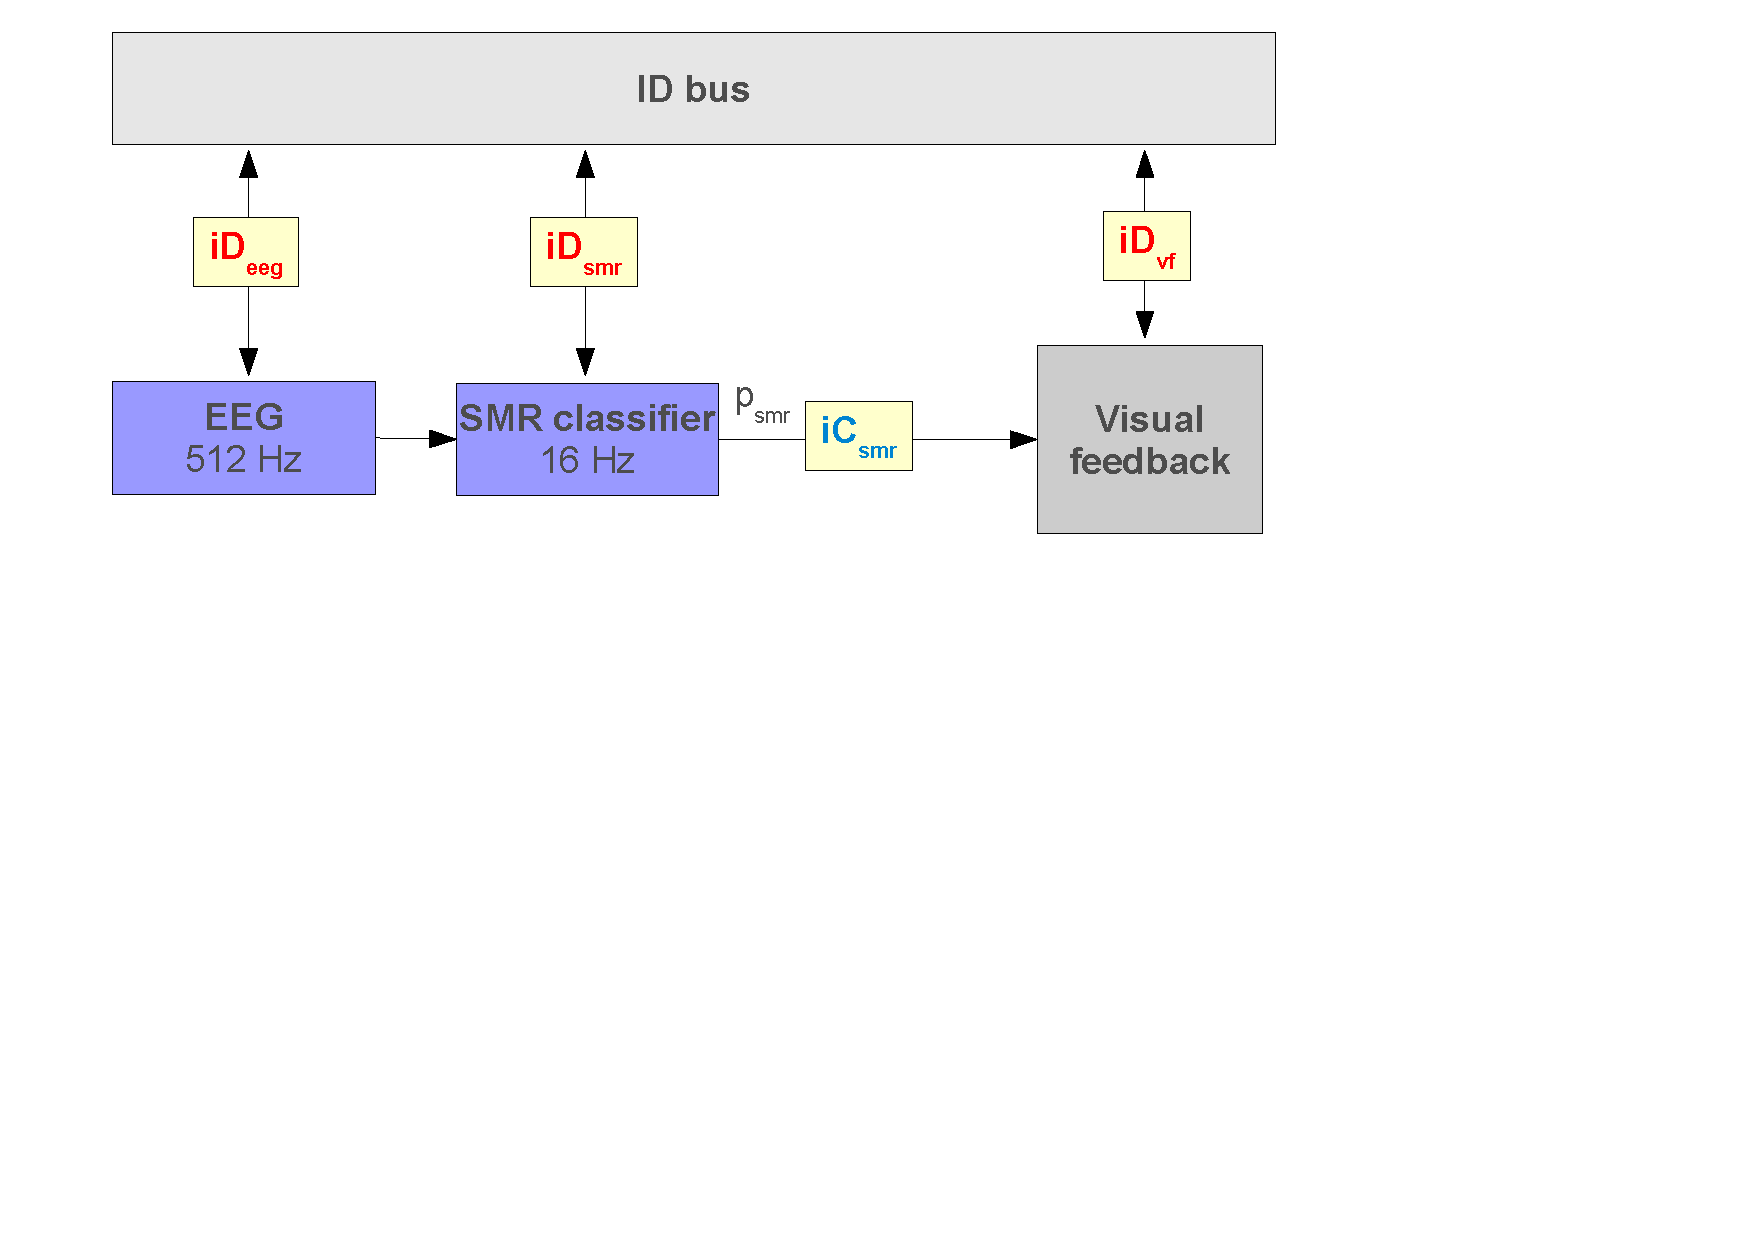
\includegraphics[width=\textwidth]{figures/example1.pdf}
	\caption{}
	\label{fig:hbci:single}
  \end{center}
\end{figure}
In this particular example: 
$f_{hBCI} = 16 Hz$ and $T_{hBCI} = (16 Hz)^{-1} = 0.0625 s$.
We will also assume that each module checks for the presence of iD messages
(vertical bidirectional arrows) continuously. The reader can imagine that each
module is able to receive, parse and process iD events in multi-threaded
fashion.

Let's now imagine that, every now and then, the visual feedback module raises an
event, with the intent to notify the SMR classifier about its status. 
For example: the feedback module writes an event on the iD bus at frame $F_n$.
All the other modules will receive immediately the event, reacting accordingly.
Typically, the EEG module will write immediately the event to some kind of file.
Similarly, the SMR classifier will react (i.e. changing the weights of an LDA
classifier) so that at frame $F_{n+1}$ the feedback module can receive and
updated classifier output.

\subsubsection*{The importance of frame numbers}
When a module in the hBCI assembly receives an iD message, it must compare the
frame number of the iD message with the frame number of its iA or iC input.
This is particularly crucial to access when and where a message was generated.
If we assume that the whole hBCI pipeline can process data in real time (that is
within $1/f_{hBCI}$ seconds), than any module can receive iD messages just from
modules processing the very same EEG frame.

If the realtime assumption does not hold, things get more complicated. Let's
consider a module $M$ that at frame $I$ receives an iD message from a module
$K$ processing frame $J$:
\begin{itemize}
  \item $I$ = $J$: $M$ and $K$ are processing the same frame, thus the 
  realtime assumption holds (at least for these two modules)
  \item $I$ > $J$: $M$ is $I-J$ frames ahead $K$. This means that a module is
  introducing a delay between modules $M$ and $K$. It also means that module $M$
  precedes module $K$ in the hBCI pipeline, or, according to
  Figure~\ref{fig:hbci:single} and~\ref{fig:hbci:multiple}, $M$ is on the left
  of $K$.
  \item $I$ > $J$: $M$ is $J-I$ frames behind $K$. This means that a module is
  introducing a delay between modules $K$ and $M$. It also means that module $M$
  succeeds module $K$ in the hBCI pipeline, or, according to
  Figure~\ref{fig:hbci:single} and~\ref{fig:hbci:multiple}, $M$ is on the right
  of $K$.
\end{itemize}

\subsection{hBCI and multiple pipelines}
\label{sec:hbci:multiple}
The example in Section~\ref{sec:hbci:single} describes how iD messages are
exchanged in a simple BCI. 
The difference between a BCI and an hBCI has to be found in the multiple
processing pipelines of the latter.
Figure~\ref{fig:hbci:multiple} shows an hBCI that acquires a single biological
signal (EEG) to classify SMRs and ErrPs. 
\begin{figure}[!h]
  \begin{center}
	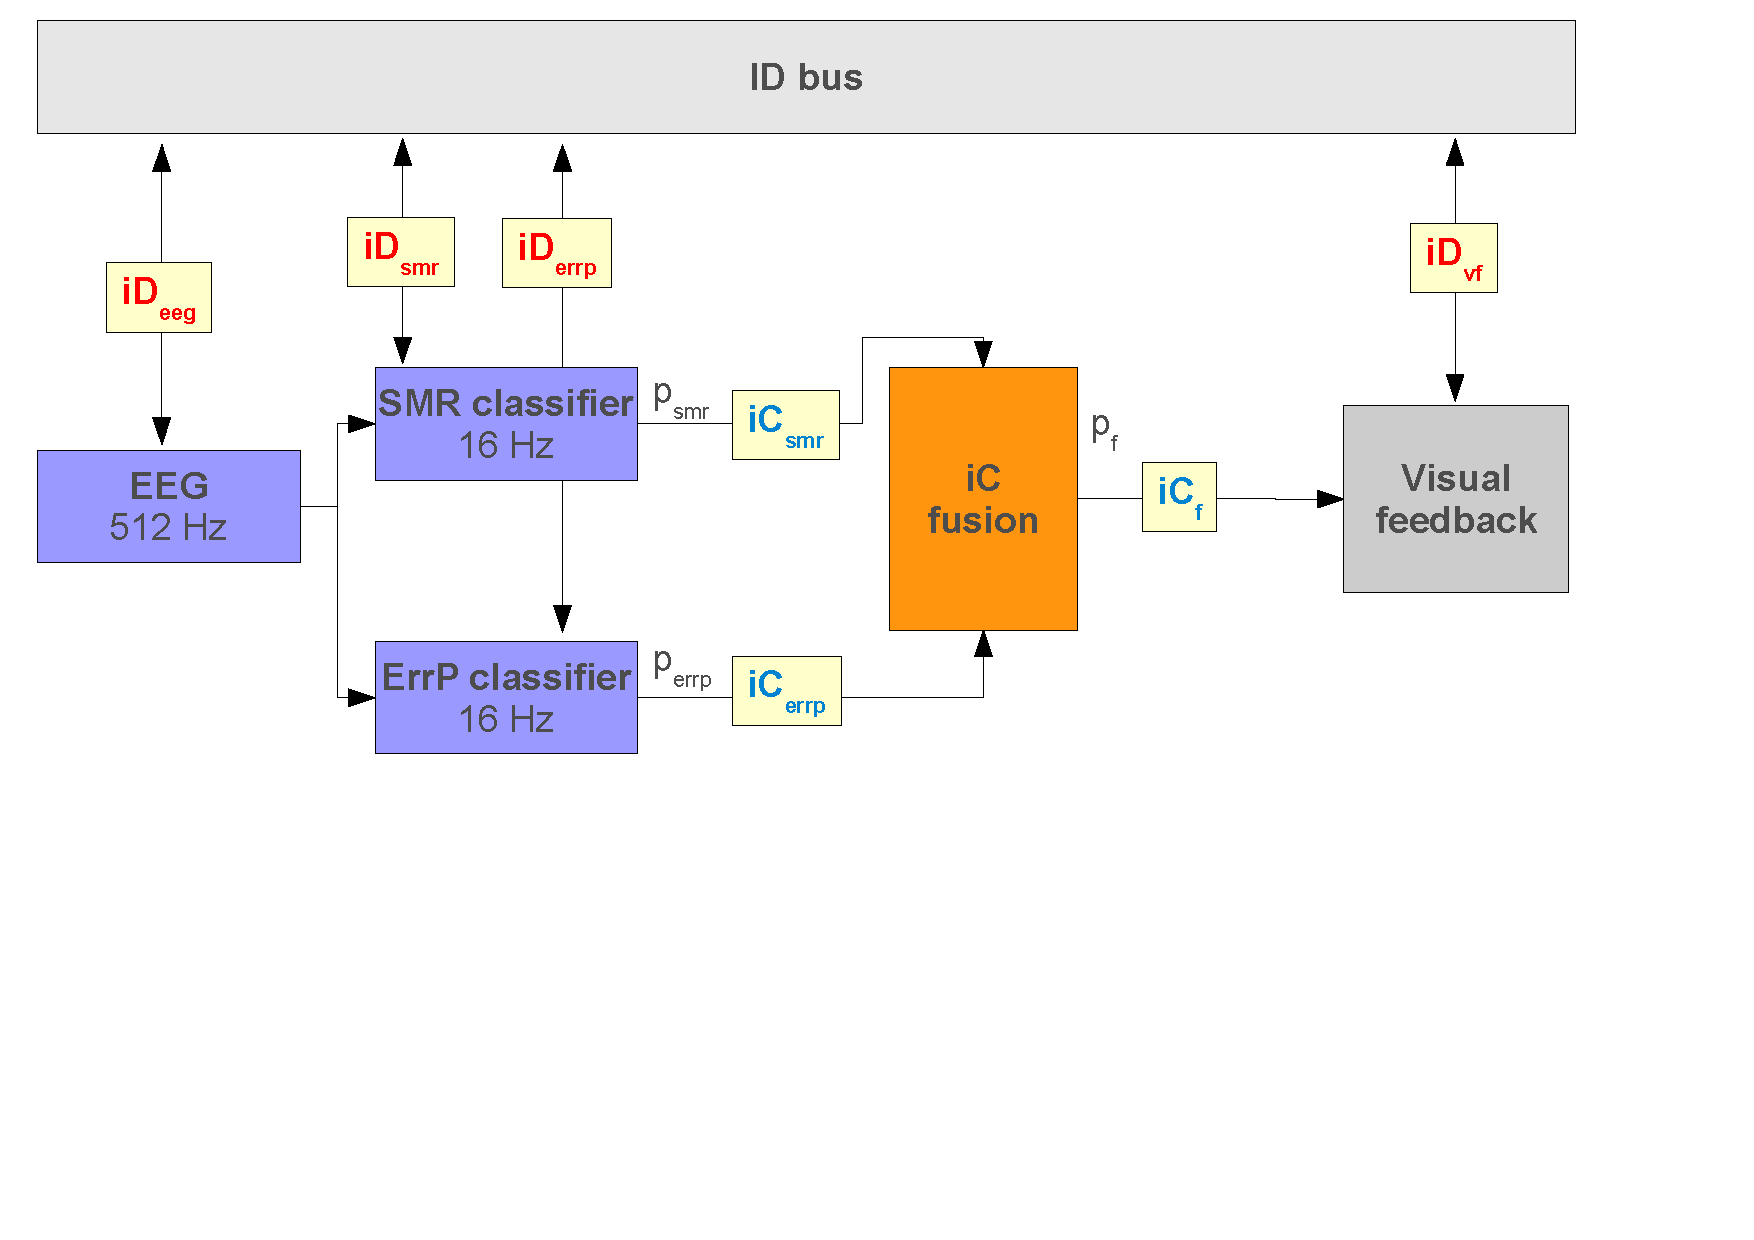
\includegraphics[width=\textwidth]{figures/example2.pdf}
	\caption{A prototypical hBCI in which the output of multiple pipelines 
	(\temp{$iC_{smr}$} and~\temp{$iC_{errp}$}) are fused in a single one
	(\temp{$iC_{f}$}).}
	\label{fig:hbci:multiple}
  \end{center}
\end{figure}
In this case the EEG acquisition sends data frames both to the SMR and to the
ErrP classifiers.
As seen before, all modules can be interfaced with the iD bus, thus being able
to send and receive messages.
A core component of the hBCI is the fusion module. A fusion module receives
multiple iC inputs and merge them in a single output, that is than transmitted
to higher-level modules.
With respect to iD and frame numbers, the fusion module carries the burden of
aligning the input iC messages in time, thus to provide a consistent iC output.
This becomes particularly critical when one of the input modules (i.e. SMR or
ErrP) is delayed in time or when the input modules are producing iC outputs at
different rates. 

\section{Structure of an iD message}
\label{sec:idstructure}
iD messages are used to transmit events withing the hBCI assembly.
Figure~\ref{fig:hbci:ismessage} depicts the attributes of an iD message.
\begin{figure}[!htb]
  \begin{center}
	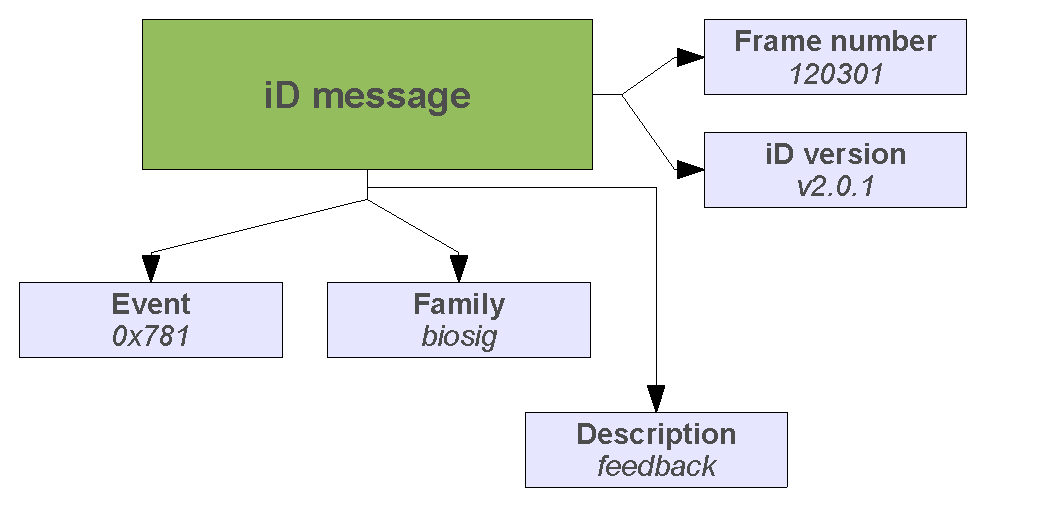
\includegraphics[width=\textwidth]{figures/idmessage.pdf}
	\caption{Internal structure of an iD message. The light blue boxes contain
	the attributes.}
	\label{fig:hbci:ismessage}
  \end{center}
\end{figure}
The attributes of an iD message are straight forward. Frame number and iD
version are used to encode temporal information and libtobiid version number
respectively.
The main content of an iD message has to be found in the event code and in its
family label. As today iD supports only Biosig and custom family types.


\section{Implementation}
\label{sec:implementation}

\subsection{Communication}
\label{sec:transport}
As today iD is not shipped with a transport layer (i.e. TCP/IP, UDP) because
different partners within the TOBI consortium use already different networking
stacks. 
If you are not expert in coding and you want to evaluate iD, we strongly
recommend to start with the MEX interface and eventually using jtcp or judp for
sending data on the network.

\subsection{Serialization}
\label{sec:serialization}
Up to now we always said that iD messages are exchanged between different
modules. Still, we never addressed specifically how this messages are encoded
and decoded for the transmission.
Similarly to what has been said in Section~\ref{sec:transport} for the
communication, different groups might require different solutions for
encoding/decoding iD messages.
For this reason the library provides a template class named \emph{IDSerializer}
on top of which is possible to implement any serialization method.

As today the consortium agreed on keeping the complexity of high-level
communication as low as possible, thus choosing XML (using RapidXML as a
back-end) for the serialization and de-serialization of the iD messages.
Readers interested in this topic will find all the necessary informations in
Section~\ref{sec:examples}.

Some examples of serialized iD messages are available in
Section~\label{sec:code:single}.

\subsection{libtobiid}
\label{sec:libtobiid}
The C++ library is distributed with a Doxygen API documentation and several
examples. It can be downloaded from here: \small{\texttt{http://}}.

\subsection{mextobiid}
\label{sec:mextobiid}
The MEX interface is distributed with the standard Mathworks Matlab
documentation and several examples. It can be downloaded from here:
\small{\texttt{http://}}.


\section{Examples}
\label{sec:examples}
An example coded in Matlab is hereby provided to illustrate how iD messages can
be handled and how certain operation on frame numbers can be performed.
The example resembles what has been described in Section~\ref{sec:hbci}. 

The following are the main functional blocks within the provided example:
\begin{itemize}
  \item Lines 19-32: configuration of iD as client
  \item Lines 42-45: configuration of an iD message as sent from a classifier
  module
  \item Lines 47-50: configuration of an iD message as sent from a feedback
  module
  \item Lines 52-55: configuration of a delayed iD message
  \item Lines 57-69: in these lines the iD events and the frame numbers are
  assigned. Furthermore, the messages are added to the client queue
  \item Lines 71-86: dequeuing of iD messages coming from modules that precede
  the simulated one
  \item Lines 88-103: dequeuing of iD messages coming from modules that succeed
  the simulated one.
  \item Lines 99-102: detection of iD messages transmitted from delayed modules
\end{itemize}
An XML message resulting from the iD serialization can be found in
Section~\ref{sec:code:xml}.
\lstinputlisting{mat/example1.m}

\subsection{XML message}
\label{sec:code:xml}
The reader can refer to Section~\ref{sec:idstructure} for interpreting the
different attributes of the XML message.
\lstinputlisting{xml/example.xml}


\end{document}
